\chapter{Deep Learning for NLP}

{\sf Working with emages is quite simple in terms of image is already a vector or a tensor and you can just put it into your network. But words are more complicated. What is the word? Word is some sequence of letters with meaning. And close sequences can have opposite meanings. What we want to do is we still want to have a vector what we can feed into the neural network. And that is achived in word embeddings.}

\section{Word Embeddings}

Word embedding is creating vector representation for words from dictionary [обычно размерность пространства таких векторов берется в районе 100-300]. For example, we can create the vector space when some pathes have meaning: we take word <<queen>>, subtract the word <<woman>>, add the word <<man>> and end up with the vector of word <<king>>. Let's demonstrate how to achieve that.

\subsubsection*{word2vec (Google 2013)}

To create the vector from word we need some task that this vector should achieve. For example we can predict what words may surround a specific word $w_c$:
$$P(w_t|w_c)=\frac{e^{f(w_t,w_c)}}{\sum\limits_{w_i\in Dict}e^{f(w_i,w_c)}}$$
where $P(w_t|w_c)$ means the probability that some word $w_t$ is near the word $w_c$ ($f$ is some function). So after that we can calculate the loss function $J$:
$$J(w_c, T)=\frac{1}{|T|}\sum\limits_{w_t\in T}J_t,\qquad J_t=-\log P(w_t|w_c)=-f(w_t,w_c)+\log\Big(\sum\limits_{w_i\in Dict}e^{f(w_i,w_c)}\Big)$$
where $w_t$ are words in some neighborhood $T$ of word $w_c$. For example, in sentence <<Quick brown fox jumps over the lasy dog>> words <<quick>>, <<brown>>, <<jumps>> and <<over>> are neighbors for the word <<fox>>. So the word2vec method is let
$$f(w_t,w_c)=u_{w_t}^Tv_{w_c}$$
where $u$ and $v$ are word embeddings for words $w_t$ and $w_c$. Also every word $w$ has two vectors: one for calculations when $w$ is the target word (the first parameter of $f$) and one when $w$ is a center word (the second parameter of $f$). So we can initialize all vectors randomly and than shift them into correct ones by using gradient ascent. NOT descent, because we want to maximize the loss function! The terminology sometimes shifts...\\
But word2vec has a problem: every time we calculate the loss funcrion we need to sum up over all words in dictuary. Instead of that we can just select 5-10 samples of negative examples and sum up over them. This kind of word2vec is used in CBOW and skip-gram. In the first one we try to predict the word from the sum of the vectors of the surrounding words (to predict the center words from the contex). And the second one is trying to predict the context from the center word.

\subsubsection*{Fasttext}

A good increase in embeddings was fasttext from Facebook. They moved from embedding just for word to having the sum of embeddings for the word and all its possible n-gramms:
\begin{center}
	where $\to$ <where> + <wh + whe + her + ere + re>
\end{center}
where '<' and '>' are starting and ending symbols. This allows to have embeddings for that words what we did not encounter in our training process: embedding of a new word will be just a sum of embeddings of its n-gramms [да, без первого слагаемого, представляющего embedding всего слова целиком]. Also the number of n-gramms is much much less than number of words in a dictionary.

\subsubsection*{Sentence embedding}

It is still the same, you try to predict the next sentence from the vectors of words or you can just use sentence as the word.
The second way also works for protein sequences. They separated into 3-gramms in 3 ways: when you start from the first letter, the second and the third:
$$^{\color{red}(1)}M^{\color{blue}(2)}A^{\color{green}(3)}FSAEDVLKEYDRRRRMEAL..$$
$$\begin{cases}
	{\color{red} 1)} & MAF,SAE,DVL,KEY,DRR,RRM,..\\
	{\color{blue} 2)} & AFS,AED,VLK,EYD,RRR,RME,..\\
	{\color{green} 3)} & FSA,EDV,LKE,YDR,RRR,MEA,..\\
\end{cases}$$
So if you reduce dimensionality of received vectors, put 3-gramms on a map and paint them according to some chemical or phisical properties, you will see that it is able to extract the fisical or chemical information, for example, same mass, polarity etc:\\
\begin{figure}[h]
  \centering
  \begin{tabular}{ccc}
    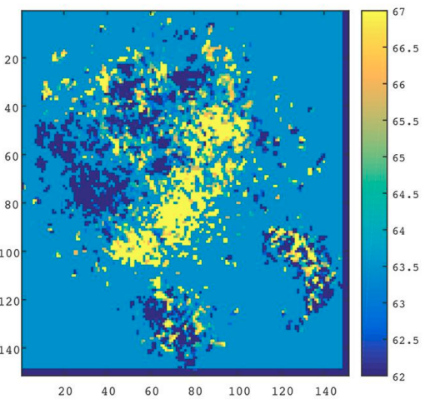
\includegraphics[width=0.25\linewidth]{8a.png} & \hspace{0.5cm}
    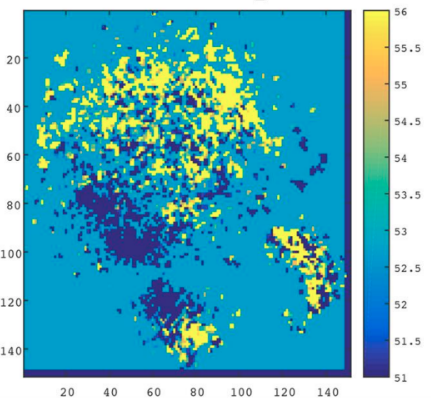
\includegraphics[width=0.25\linewidth]{8b.png} & \hspace{0.5cm}
    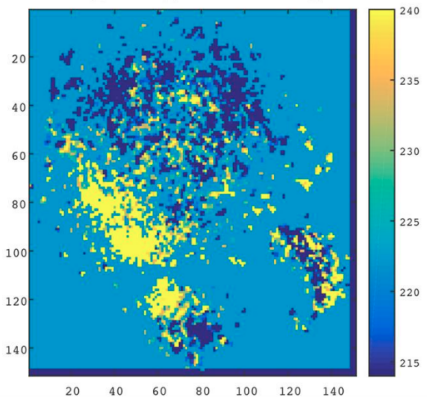
\includegraphics[width=0.25\linewidth]{8c.png} \\
    Mass & Polatiry & Hydrophobicy \\
  \end{tabular}
\end{figure}
That's amazing because you don't actually tell the computer that theese are protheins with letters correspondes to some chemical properties.

\section{Models in NLP}

The important thing is you don't have to use neural networks after you get embeddings. After you use deep learning technics to obtain your vectors you can use your vectors in trees or kNN etc. But if you want to do something complicated like mashine learning translation or text generation, you can use recurrent neural networks (RNN).

\subsubsection*{RNN}

The H's are networks, x's are inputs and y's are outputs [pic. 8.1]. Each network in RNN does not only produce an output but also some vector that it fits in the next same network. And for two years everyone got excited about recursive neural networks [pic. 8.2] but not anymore.\\
\begin{figure}[h]
  \centering
  \begin{subfigure}[c]{0.5\linewidth}
    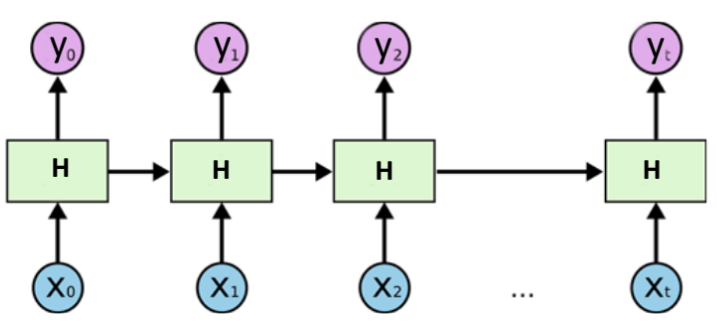
\includegraphics[width=\linewidth]{8d.png}
    \caption*{(8.1) Recurrent NN}
  \end{subfigure}
  \hspace{2cm}
  \begin{subfigure}[c]{0.3\linewidth}
    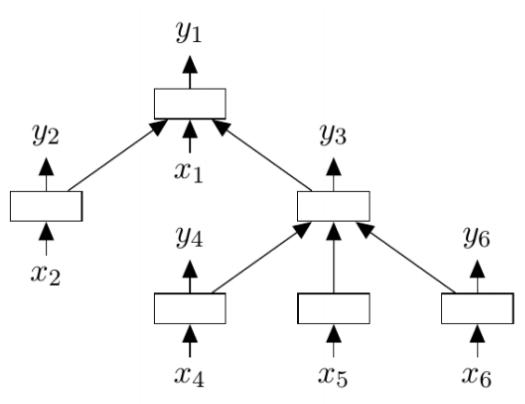
\includegraphics[width=\linewidth]{8e.png}
    \caption*{(8.2) Recursive NN}
  \end{subfigure}
\end{figure}
But the problems show themselves quite quickly after we start using RNNs and the almost always we have to do with vanishing or exploding gradient. {\it <The intuition why it happens>} To fight that the LSTM was envented.

\subsubsection*{LSTM, BiLSTM}

LSTM is a long short term memory network (we are going to go in depth over that network in a deep learning cource). What we need to know by now: it may helps when you have a sequentional data. The important thing is LSTM decides on each step what to keep from previous step, what to keep from current input and what to keep from current output.
\begin{wrapfigure}{r}{0.35\linewidth}
  \vspace{-1.4cm}
  \begin{center}
    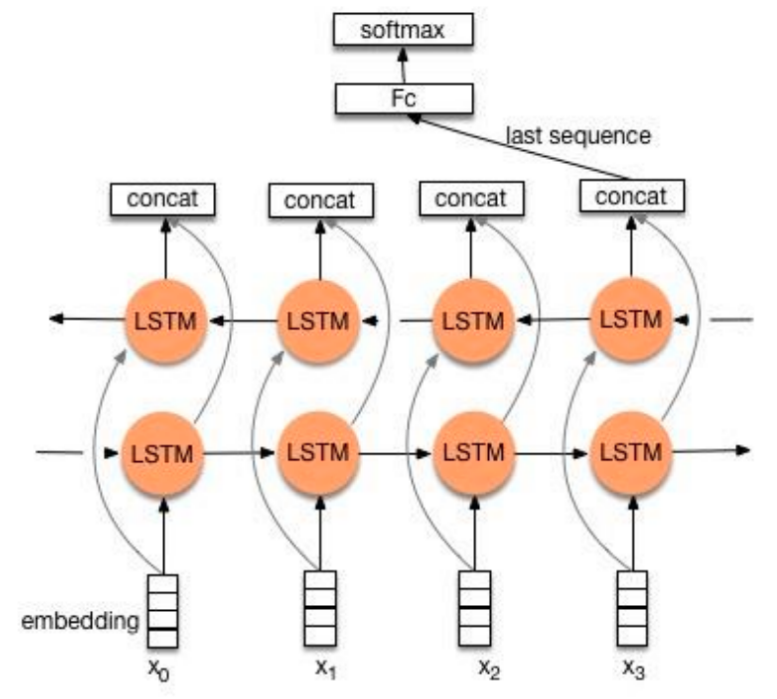
\includegraphics[width=\linewidth]{8f.png}
  \end{center}
  \vspace{-0.6cm}
  \caption*{(8.3) BiLSTM}
  \vspace{-0.8cm}
\end{wrapfigure}
How does LSTM looks in practice? It is a BiLSTM (bidirectional LSTM) [pic. 8.3]. Every word represented as a vector feeds into the first LSTM network and then you have another LSTM network what goes into other direction. So you read the text from front to back and from back to front and then feed outputs from the first network to the second. Then you concatenate both outputs and the result is a desicion for something. For example, if you want to generate the next word you can use softmax for the dictionary and then select the maximum. This is common used LSTM structure because you get more information when you go from left to right and from right to left.

\subsubsection*{Attention}

\begin{wrapfigure}{r}{0.35\linewidth}
  \vspace{-1cm}
  \begin{center}
    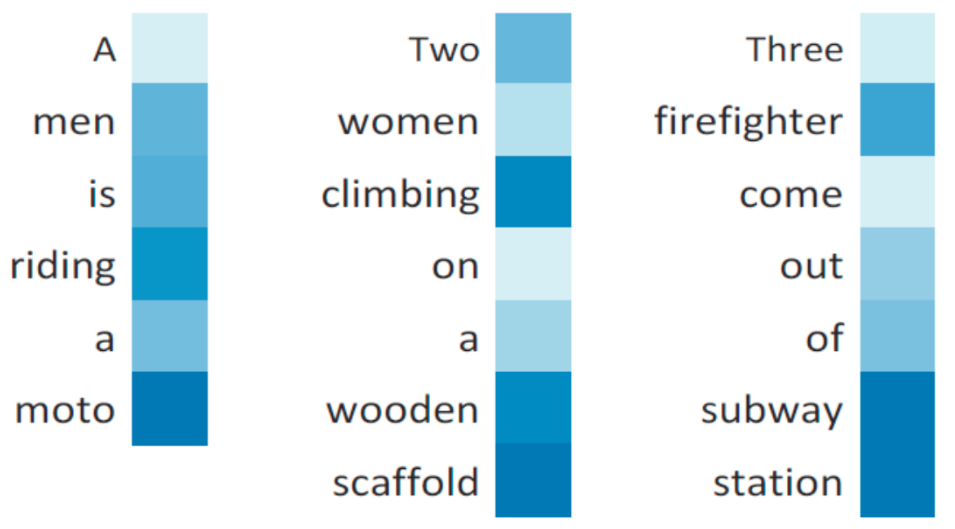
\includegraphics[width=\linewidth]{8g.png}
  \end{center}
  \vspace{-0.6cm}
  \caption*{(8.4) Attention}
  \vspace{-0.6cm}
\end{wrapfigure}
Attention is just adding a layer with the softmax after input layer. The property of the vector you get from softmax is that all the numbers of the features are summed up to one. It is called attention because you try to see how much attention every input gets. So you put your input into the attention layer, then you multiply the output of the attention network by the input and then you feed the result into desicion network. Here [pic. 8.4] you can see examples of distribution attention in a sentence. This picture does not show that men is more important than woman! The attention has meaning only in one sentence: <<climbing>> has more attention then <<two>> because it is more important for our decision. 

\subsubsection*{Transformers}

Transformers is a way to encode positional information and relationship. They have levels of input abstractions: query (Q), key (K) and value (V). For some tests your input is a query and key, sometimes it's value. We projected Q, V, K to various linear neural networks [идея в том, чтобы посмотреть на входные данные с разных сторон]. After that we use an attention to know how important is what we projected.\\
Another thing is a positional encoding. Positional encoding is adding some numbers to the input. Inputs with close positional encodings are close to each other and different positional encodings are far away from each other. You don't always have to use positional encodings. Sometimes it helps, sometimes it doesn't.

\section{Translation}
\vspace{-0.6cm}
\subsubsection*{Google neural machine translation}

How the mashine translation works now such as a Google mashine translation? Every time you write something to Google to be translated, your phrase goes into the eight GPUs (right now maybe more) and encoded into one vector that captures the meaning of the phrase. And that you decode that vector into another language one word by one. In this case you need examples of translations (parallel texts) for training.

\subsubsection*{Transation without parallel texts}

Facebook made very cool thing a couple mounthes ago. How to get translations if you don't have examples? How did they do that? They tried to push embeddings together. So you have one embedded space, you have another embeded space and let's made them look alike. Then we can switch a word embedding: one embedded language makes a vector from that word and another just decodes the result. How to push embeddings together?

\vspace{-0.3cm}
\subsubsection*{Adversarial learning}

Adversarial learning is when you work against another network. [Используется $N$ сетей, одна для каждого языка. Каждая сеть -- автоэнкодер, т.е. пытается на выходе получить ту же фразу, что и на входе. В середине этих сетей расположен слой небольшого размера, веса которого образуют embedding для фразы с input'а. Еще одна сеть, adversarial, смотрит на embedding вектора с этих слоев и пытается определить, к какой сетке (и, соответственно, к какому языку) они относятся. Ее награда (функция, которую мы максимизируем) -- то, насколько правильно она классифицирует. Награда каждой из $N$ сетей-автоэнкодеров -- сумма того, насколько она правильно восстанавливают фразу, и награды adversarial сети со знаком минус. Т.е. они помимо своей задачи восстановления последовательностей ище и стараются, чтобы вектора embedding были похожи. После обучения перевод из языка A в язык B выглядит следующим образом: мы берем первую половину сети-автоэнкодера для языка A и правую половину сети-автоэнкодера для языка B и конкатенацией получаем сеть, переводящую фразу.]

\vspace{-0.3cm}
\subsubsection*{Image Captioning}

The image captioning is just a translation from image to text. You have an images, you have a number of features and you decode that vector into text.